%%
\documentclass[journal]{IEEEtran}
\usepackage[pdftex]{graphicx}
\usepackage[cmex10]{amsmath}
\usepackage{amssymb}
\usepackage{caption}
\usepackage{subcaption}
\usepackage{cite}
\usepackage{epstopdf}
\usepackage{color}
\usepackage{multirow}
\usepackage{hyperref}
\usepackage{graphicx,booktabs,array}
\usepackage[dvipsnames]{xcolor}
\newcommand{\addpic}{\includegraphics[width=6em]{example-image}}
\newcolumntype{C}{>{\centering\arraybackslash}m{6em}}
% \DeclareGraphicsExtensions{.pdf,.jpeg,.png}
% *** GRAPHICS RELATED PACKAGES ***
%
\ifCLASSINFOpdf
  % \usepackage[pdftex]{graphicx}
  % declare the path(s) where your graphic files are
  % \graphicspath{{../pdf/}{../jpeg/}}
  % and their extensions so you won't have to specify these with
  % every instance of \includegraphics
  % \DeclareGraphicsExtensions{.pdf,.jpeg,.png}
\else
  % or other class option (dvipsone, dvipdf, if not using dvips). graphicx
  % will default to the driver specified in the system graphics.cfg if no
  % driver is specified.
  % \usepackage[dvips]{graphicx}
  % declare the path(s) where your graphic files are
  % \graphicspath{{../eps/}}
  % and their extensions so you won't have to specify these with
  % every instance of \includegraphics
  % \DeclareGraphicsExtensions{.eps}
\fi
% correct bad hyphenation here
\hyphenation{op-tical}
\begin{document}
%
% paper title
% can use linebreaks \\ within to get better formatting as desired
\title{On the Achievable Capacity\\ of Multi-band Optical Line Systems}
%
%
% author names and IEEE memberships
% note positions of commas and nonbreaking spaces ( ~ ) LaTeX will not break
% a structure at a ~ so this keeps an author's name from being broken across
% two lines.
% use \thanks{} to gain access to the first footnote area
% a separate \thanks must be used for each paragraph as LaTeX2e's \thanks
% was not built to handle multiple paragraphs
%
\author{Alessio Ferrari, Antonio Napoli, Andrea D'Amico, Johannes K. Fischer, Nelson Costa, Jo\~ao Pedro, Erwan Pincemin, Wladek Forysiak, Chris Matrakidis, Gunther Roelkens, Juan Pedro F.-P. Gimenez\\ Silvio Abrate, Nicola Calabretta, Vittorio Curri, Bernd Sommerkorn-Krombholz
\thanks{This work was partially funded by the German BMBF, contract no. 16KIS0487K (Celtic project SENDATE-FICUS) and by the H2020 Metro-Haul project, grant agreement no. 761727.}
\thanks{Alessio Ferrari, Andrea D'Amico and Vittorio Curri are with Politecnico di Torino, Torino, Italy, alessio.ferrari@polito.it.}
\thanks{Antonio Napoli and Bernd Sommerkorn-Krombholz are with Infinera, Sankt-Martin-Str. 76, 81541, Munich, Germany, ANapoli@infinera.com.}
\thanks{Johannes K. Fischer is with Fraunhofer Institut HHI in Berlin, Germany.}
\thanks{Nelson Costa and Jo\~ao Pedro are with Infinera, Lisbon, Portugal. Jo\~ao Pedro is also with Instituto de Telecomunica\c{c}{o}es, IST, UL, Lisbon, Portugal.}
\thanks{Erwan Pincemin is with Orange, Lannion, France.}
\thanks{Juan P. F.-P. Gimenez is with Telefonica, Madrid, Spain.}
%\thanks{Andrew Lord is with British Telecommunications, Ipswitch, UK.}
\thanks{Silvio Abrate is with ISMB, Torino, Italy.}
\thanks{Nicola Calabretta is with TU/e, Eindhoven, The Netherlands.}
\thanks{Wladek Forysiak is with Aston, UK.}
\thanks{Chris Matrakidis is with University of Peloponnese, Greece.}
\thanks{Gunther Roelkens is with Gent University, Belgium.}

\thanks{Manuscript received xxx 19, zzz; revised January 11, yyy.}}
% note the % following the last \IEEEmembership and also \thanks -
% these prevent an unwanted space from occurring between the last author name
% and the end of the author line. i.e., if you had this:
%
% \author{....lastname \thanks{...} \thanks{...} }
%                     ^------------^------------^----Do not want these spaces!
%
% a space would be appended to the last name and could cause every name on that
% line to be shifted left slightly. This is one of those "LaTeX things". For
% instance, "\textbf{A} \textbf{B}" will typeset as "A B" not "AB". To get
% "AB" then you have to do: "\textbf{A}\textbf{B}"
% \thanks is no different in this regard, so shield the last } of each \thanks
% that ends a line with a % and do not let a space in before the next \thanks.
% Spaces after \IEEEmembership other than the last one are OK (and needed) as
% you are supposed to have spaces between the names. For what it is worth,
% this is a minor point as most people would not even notice if the said evil
% space somehow managed to creep in.
% The paper headers
\markboth{JOURNAL OF LIGHTWAVE TECHNOLOGY, VOL. xxxx, NO. yyyy, wwww hhh, zzzz}%
{Shell \MakeLowercase{\textit{et al.}}: On the Achievable Capacity for Multi-band Optical Systems}
% The only time the second header will appear is for the odd numbered pages
% after the title page when using the twoside option.
%
% *** Note that you probably will NOT want to include the author's ***
% *** name in the headers of peer review papers.                   ***
% You can use \ifCLASSOPTIONpeerreview for conditional compilation here if
% you desire.
% If you want to put a publisher's ID mark on the page you can do it like
% this:
%\IEEEpubid{0000--0000/00\$00.00~\copyright~2007 IEEE}
% Remember, if you use this you must call \IEEEpubidadjcol in the second
% column for its text to clear the IEEEpubid mark.
% use for special paper notices
%\IEEEspecialpapernotice{(Invited Paper)}
% make the title area
\maketitle
\begin{abstract}
Multi-band (MB) optical systems transmit over all low-loss bands of a single-mode fibre (SMF). This spectrum ranges from 1260~nm to 1625~nm, covering $\sim$55~THz, which is $\sim$10 times the C-band. This solution is realistic because the most of the deployed fibers consists of the ITU-G.652D, which presents a negligible absorption peak at $\sim$1380~nm. Consequently, MB can significantly increase the fiber capacity and thus efficiently utilizing the existing telecommunication infrastructures. The latter represents the main advantage compared to the well established multi-mode or -core approaches. Furthermore, the industrial trend is clear: First commercial C+L-band systems are entering the market and research started considering the neighbor S-band. However, fundamental components such as the amplifiers and full spectrum tunable lasers are not mature yet.\\
In this contribution, we discuss the potentialities and challenges for the realization of MB systems transmitting from O$\rightarrow$L-band and we assess, by employing the generalized Gaussian-noise (GGN) model, the performance of such system for several scenarios and configurations. For example, we considered options such as turning off the O-band, to place Raman pumps to amplify the E-band.\\
We estimate a total fiber capacity for DCI as high as 450~Tb/s/fiber over 75~km in presence of stimulated Raman scattering (SRS). In case of metro and regional scenarios, capacities well above 200~Tb/s/fiber are achievable, i.e., a factor $\times$10 improvement compared to commercial systems.
\end{abstract}
% IEEEtran.cls defaults to using nonbold math in the Abstract.
% This preserves the distinction between vectors and scalars. However,
% if the journal you are submitting to favors bold math in the abstract,
% then you can use LaTeX's standard command \boldmath at the very start
% of the abstract to achieve this. Many IEEE journals frown on math
% in the abstract anyway.
% Note that keywords are not normally used for peerreview papers.
\begin{IEEEkeywords}
    Multi-band transmission, high-capacity systems, elastic optical networks, wideband amplifiers
\end{IEEEkeywords}
% For peer review papers, you can put extra information on the cover
% page as needed:
% \ifCLASSOPTIONpeerreview
% \begin{center} \bfseries EDICS Category: 3-BBND \end{center}
% \fi
%
% For peerreview papers, this IEEEtran command inserts a page break an
% creates the second title. It will be ignored for other modes.
\IEEEpeerreviewmaketitle
%                       %
%       **********      %
%       **********      %
%                       %
\section{Introduction}\label{Sec:Intro}
\IEEEPARstart{B}{efore} the advent of coherent, direct-detection systems could generate throughput $<$~1~Tb/s/fiber at 10 Gb/s/ch. Nowadays, current commercial transponders can transmit up to 38.4~Tb/s/fiber with 600~Gb/s/ch polarization multiplexing 64-quadrature amplitude modulation (PM-64QAM) formats~\cite{Infinera600G}. However, this improvement might not be sufficient to cope with the current IP traffic demand, which in 2017 reached an average compound annual growth rate of $\sim$24\%~\cite{Cisco_2017}. Higher values have been estimated for metro and data center interconnect (DCI). In addition, the imminent deployment of 5G and high-capacity access networks will further stress the existing optical network infrastructures. To cope with this scenario, research identified two possible approaches: spatial division multiplexing (SDM) and multi-band transmission (MBT). Both are already partially commercially available.\\
\emph{SDM} is implementable in several ways: \textbf{I)} By utilizing the available dark fibers~\cite{winzer2018scaling} (i.e., multi-fibers (MF)). This is preferred choice; II) By deploying new ones in the same duct. This is still optimal; III) By rolling out new single mode fiber (SMF), which is highly costly~\cite{jimenez2017techno}; and finally IV) by utilizing multi-mode / -core optical fibers (MMF and MCF), which, from one hand, showed great potential~\cite{van2014ultra, kobayashi20171}, but on the other the technology is not mature for mass deployment yet and requires new roll-outs.\\
In this context \emph{MBT} is the most affordable solution to increase fiber capacity once fibers saturate~\cite{napoli2018towards}, because by enabling transmission over the entire low-loss spectrum of single-mode fibers (SMF), it efficiently utilizes the existing network infrastructure. Fig.~\ref{fig:multi-band_definition} summarizes the different wavelength ranges for the \{O, E, S, C, L\}-band, with a spectrum in the range of $\in$~(1260~nm -- 1620~nm).

%
\begin{figure}[!htb]
\center
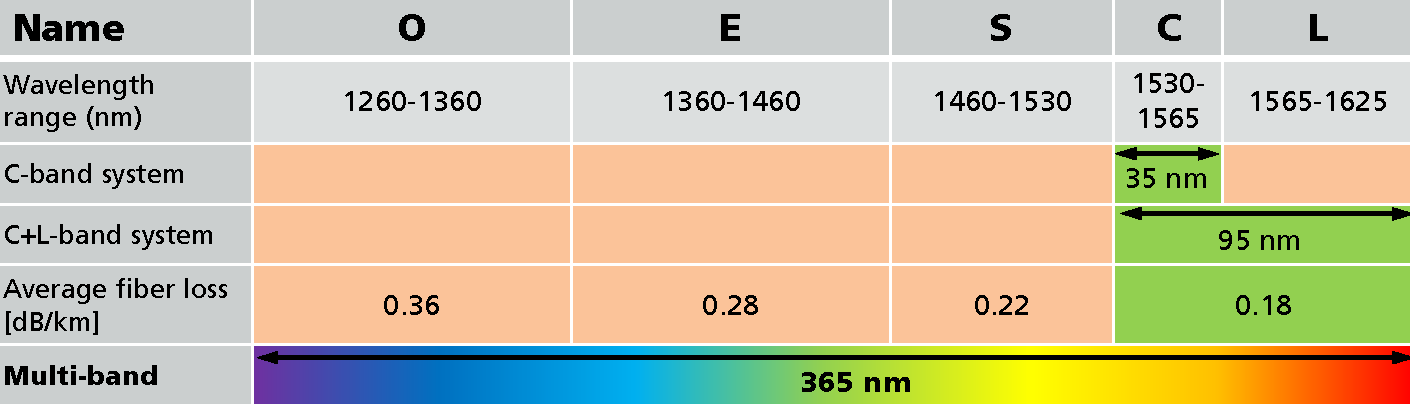
\includegraphics[width=1\linewidth]{Figures/Sec_II/Lambda_Tabelle.pdf}
\caption{Band definition and fiber attenuation of the ITU-T G.652D.}
\label{fig:multi-band_definition}
\end{figure}
%
%   
\begin{table*}[ht!]
\centering
\caption{Comparison of the strategies based on different transmission media.}
\begin{tabular}{|p{3cm}|p{3.75cm}|p{3.75cm}|p{1.5cm}|p{1.5cm}|p{1.25cm}|}
\hline
\textbf{Approach} & \textbf{Pros} & \textbf{Cons} & \textbf{Maturity} & \textbf{Capacity factor} & \textbf{Ready by 2021}\\
\hline \hline
%
\multirow{3}{*}{Multi single mode fibers} & - Mature technology & - new fiber deployment & high & depend on available fibers & certain\\ 
& - exploitation of dark fibers & - bandwidth limited & &  & \\ 
& & - larger sheath diameter & & &\\ \hline
%
\multirow{2}{*}{Multi core fiber} & high capacity & - new deployment of fibers & low & depends on available core & unlikely\\ 
& & - larger sheath diameter & & & \\ \hline
%
\multirow{3}{*}{Multi band} & - No fiber deployment & - Development of components is needed & low & & possible\\ 
& - complete usage of the bandwidth & - time need to achieve maturity & & $\times$10 & \\ 
& & - narrow diameter for the sheat & & & \\ \hline
%
%\multirow{3}{*}{Advanced devices} & Technology available & - new fiber deployment & medium & & possible\\ 
%& & - costly & & & \\
%& & - bandwidth limited & & & \\ \hline
\end{tabular} 
\label{Table:comparison}
\end{table*}
%                       %
%       **********      %
%       **********      %
%                       %
%
% from here onward
%
%
\begin{figure}[!htb]
\center
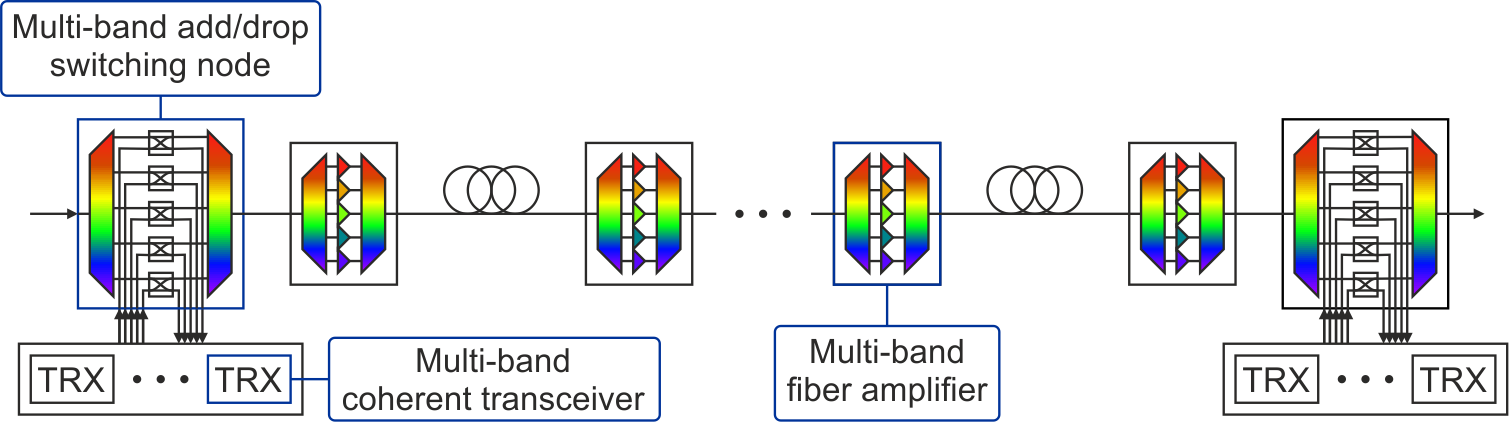
\includegraphics[width=1\linewidth]{Figures/Sec_II/EMBRACE_System.png}
\caption{Generic multi-band optical communication system}
\label{fig:system}
\end{figure}
%
\begin{figure}[!htb]
\center
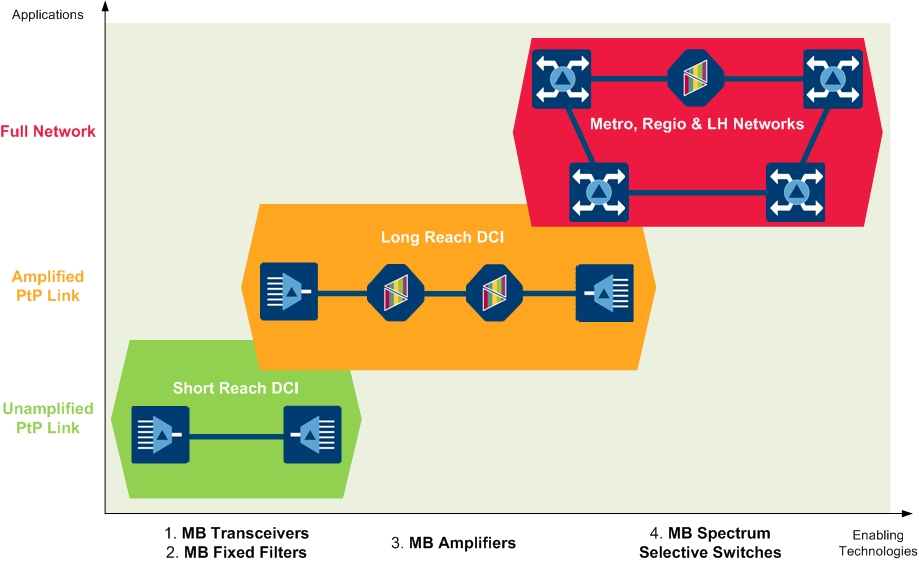
\includegraphics[width=1\linewidth]{Figures/Sec_II/MB_Tech_Evolution.jpg}
\caption{Placeholder}
\label{fig:system}
\end{figure}
%
\begin{figure}[!htb]
\center
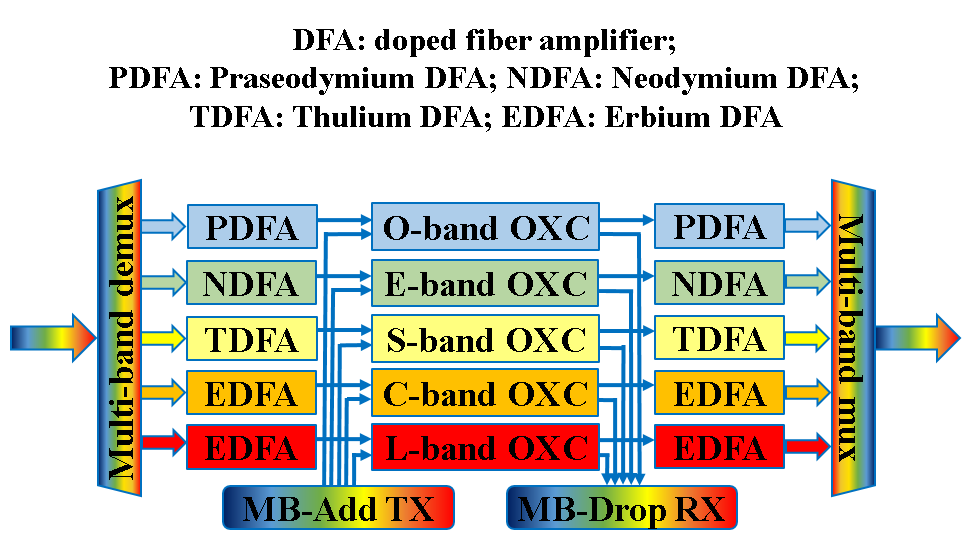
\includegraphics[width=1\linewidth]{Figures/Sec_II/ROADM_node.png}
\caption{Placeholder}
\label{fig:system}
\end{figure}
%
\section{Multi-band optical systems: potentialities and challenges}\label{Sec:MB_optical_systems}
Multi-band optical transmission presents simultaneously several potentialities and challenges, that from one hand make it a realistic solution, from another hand it might delay its first implementation. In this section, we first discuss the advantages with respect to other solutions, by providing the point of view of operators. In a second moment we highlight the requirements for the needed components and also a roadmap at system level.

\subsection{Potentialities}
The most relevant advantages of MB versus other approaches such multi-mode and/or multi-core lies on the possibility of maximizing the capacity of existing optical telecommunication infrastructures, which represents the largest part of the total cost of ownership \cite{telefonica}.\\

In fact, all recently proposed solutions

 In particular, this refers to the two differents scenarios.
In case dark fibers are not anymore available, the possibility of transmitting over bands beyond C-band

- comparison with other strategies\\

\subsection{Challenges}
- components\\

\subsection{Road-map towards multi-band systems}


\section{Multi-band transmission modelling: The generalized Gaussian Model}\label{Sec:GGN}
%
In [xxx] the authors introduced for the first time the acronym Gaussian Noise (GN) model, a concept already present in the early paper [exx], but which became ultimate only after \cite{poggiolini2014gn}. Has been verified and validated [xx] and it can be used get an easy and quick system optimization\cite{curri2015design}.\\
As shown in \cite{Filer:18} It can also be used in a quality of transmission estimator (QoT-E) up to 3 THz.
With the enlargement of the bandwidth some effects such as the Raman effect cannot be neglected. Some extension of the GN-model has been proposed to include the Raman effect \cite{curri2013extension} but it assumes a flat Raman effect in frequency. Such assumption does not hold anymore in a multiband optical system.
For this reason, a generalized Gaussian noise (GGN) model capable to take into account frequency and space variations of the signal attenuation along the fiber - including phenomena such as the stimulated Raman scattering and frequency variation of fiber attenuation - has been proposed \cite{cantono_introducing_2017,roberts_channel_2017,semrau_gaussian_2017} and validated \cite{cantono_modelling_2018, cantono_interplay_2018}.

%
%       **********      %
%       **********      %
%                       %
\section{Considered setup}\label{Sec:Setup}
\subsection{The system}
%
\begin{figure}[!htb]
\center
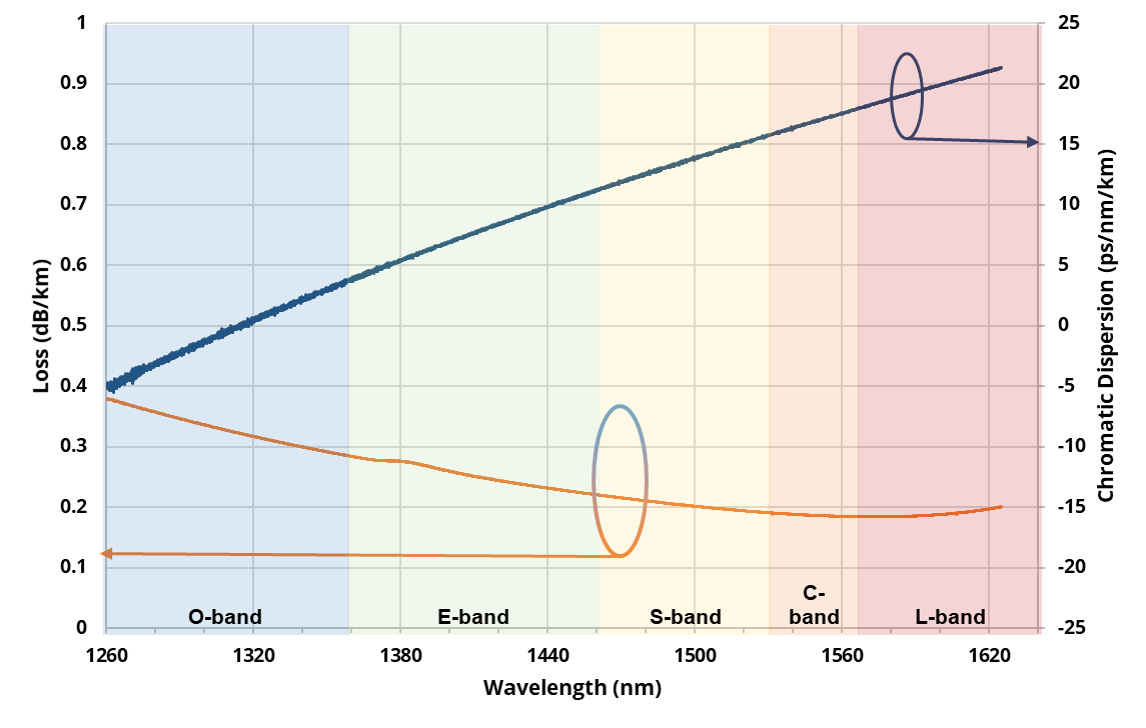
\includegraphics[width=1\linewidth]{Figures/Sec_III/fiber_parameters.png}
\caption{Measured fiber physical parameters for the ITU-T G.652D used within the GGN. Attenuation $\alpha(\lambda)$ (orange) and dispersion coefficient $D(\lambda)$ (blue).}
\label{fig:system}
\end{figure}
%
\begin{figure*}[!htb]
\center
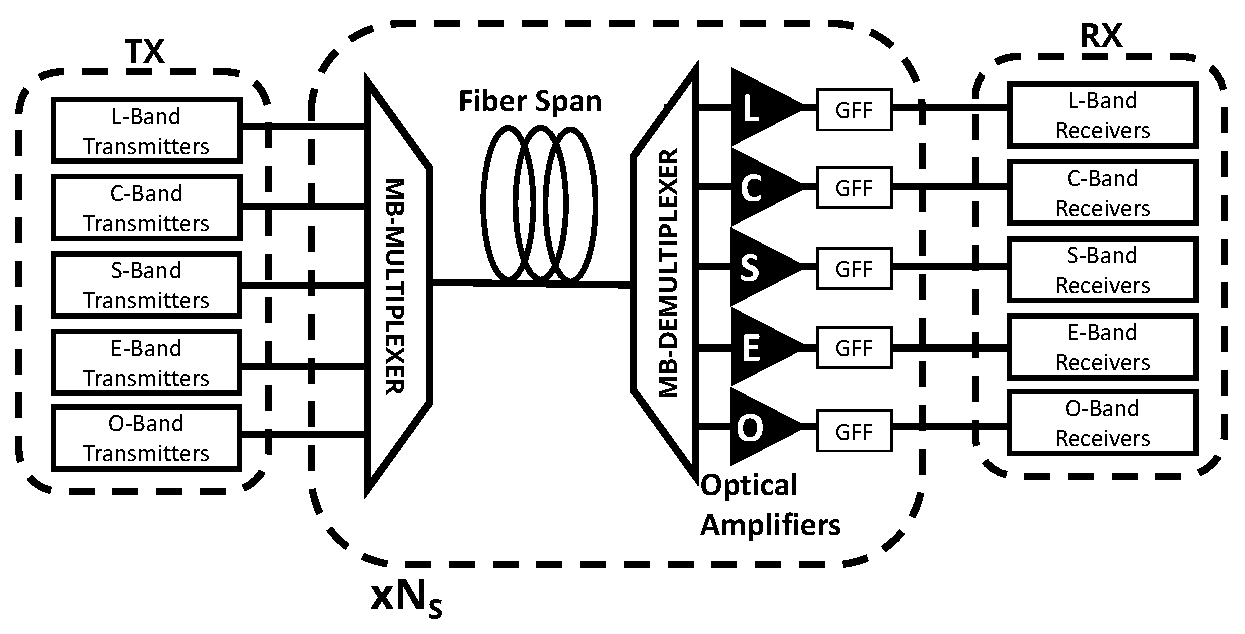
\includegraphics[width=0.5\linewidth]{Figures/Sec_III/physical_layout_v2}
\caption{Placeholder}
\label{fig:system}
\end{figure*}
%
\begin{table*}[t]
    \centering \caption{Considered parameters per each band.}
    \label{tab:params}
    \begin{tabular}{c|ccccc}
        \hline
        Parameters / Band & L & C & S & E & O \\
        \hline 
        Wavelength Range [nm] & 1565 - 1625 & 1530 - 1565 & 1460 - 1530 & 1360 - 1460 & 1260 - 1360 \\
        Number of channels & 136 & 82 & 182 & 295 & 237 \\
        Occupied Bandwidth [THz] & 6.8 & 4.1 & 9.1 & 14.75 & 11.85\\
        Central frequency [THz] & 187.96 & 193.73 & 200.53 & 212.62 &
        228.85 \\
        Amplifier's noise figure [dB] & 6 & 5.5 & 7 & 6 & 7 \\
        \hline
    \end{tabular}
    \label{tab:data}
\end{table*}
%

\begin{enumerate}
    \item Fiber type and parameters
    \item Multi-span line system
        \begin{enumerate}
            \item 50/75 km (DCI) (from OFC 2019 paper)
            \item 150 km, metro optical networks
            \item 300 km, extended metro optical networks
            \item 600 km, regional optical networks
            \item Span length: 50 km and 75 km
        \end{enumerate}
    \item Raman amplification
\end{enumerate}
\subsection{Channel power and amplifier assumptions}
\begin{enumerate}
    \item Equalization after each inline optical amplifier using gain flattening filters (i.e. the power spectral density is same at the input of each span)
    \item Flat noise figure per band
    \item Flat intraband power per channel
    \begin{enumerate}
        \item 100\% interband pre-emphasis
        \item The overall gain/loss introduced by SRS is compensated at the transmitter 
    \end{enumerate}
\end{enumerate}
\subsection{The LOGO power Optimization}
- How to compute intraband power levels:\\
    - We compute an intraband LOGO with nominal values of the system (the value at the central frequency of the band)
\subsection{Capacity maximization: a trade-off between available bands and physical effects}\label{Sec:capacity_maximization}
\subsubsection{Shannon receiver}
\subsubsection{Bands scenarios \& Raman amplifiers}
\begin{itemize}
    \item upgrade strategies
    \item Full transmission O $\longrightarrow$ L-band without Raman amplification
    \item Turn off the O band and place Raman pumps to amplify the E band (5 Raman pumps in O), Full transmission E $\longrightarrow$ L-band
    \item Turn off 0 \& E band to amplify the S band (5 Ramam pumps), full transmission S $\longrightarrow$ L-band
\end{itemize}
%                       %
%       **********      %
%       **********      %
%                       %

\section{Numerical results}\label{Sec:results}
%#
This section summarizes 
The performance will be assessed for the different distances and scenarios, by using 
\begin{itemize}
    \item Definition of: Average spectral efficiency per band which corresponds on the average bitrate for each band
    \item Total traffic per band
\end{itemize}
%                       %
%       **********      %
%       **********      %
%                       %
\section{GGN validation through Experimental C+L-band transmission}\label{Sec:Exp}
%                       %
%       **********      %
%       **********      %
%                       %
\section{Conclusion and outlook}\label{Sec:Conclusions}
The yet exploited C-band represents just a minor portion of the available spectrum of a single-mode fiber. Furthermore, the vast majority of deployed fiber does not present the water absorption peak anymore (e.g., the rending part of the single mode spectrum can be exploited for transmission in particular for high-bandwidth demand and short distances scenarios such as DCI.

%
% https://en.wikibooks.org/wiki/LaTeX/Colors
%
\pagebreak
\section{TO-DO}\label{Sec:Conclusions}
\begin{itemize}
    \item Tables
    \begin{enumerate}
        \item fiber and system parameters
        \item result summary
    \end{enumerate}
    \item Block diagrams
    \begin{enumerate}
        \item System description
        \item Fiber attenuation and dispersion with band chara
        \item ROADM
        \item WDM channel power 
        \item Considered scenarios O -> L, raman in O E -> L, etc.
    \end{enumerate}
    \item Results
    \begin{enumerate}
        \item Power evolution along the fiber vs. distance. 4 cases, 80, 150, 300, 600 km in one plot
        \item SNR of the CUT. 4 cases in one plot.
        \item Transmission capacity per band. 4 cases in one plot.
        \item Total transmission capacity. 4 cases in one plot.
        \item Average spectral efficiency per band. 4 cases in one plot.
    \end{enumerate}
\end{itemize}

\bibliographystyle{IEEEtran}
\bibliography{references}
\end{document}